
\chapter{Econometria Clássica e Efeitos Marginais}

Introduzido o conceito de Floresta Aleatória, agora voltamos nossa atenção à Econometria Clássica e seu  modelo central. Veremos uma maneira de estimar os parâmetros desse modelo via Mínimos Quadrados Ordinários, como modelos de Floresta Aleatória não têm a mesma interpretabilidade e como podemos contornar essa problemática avaliando o modelo na vizinhança de algumas observações. A apresentação seguirá \citeonline{hayashi}. 



\section{Teoria Clássica de Regressão Linear}

Retornando um pouco, e apenas esse pouco, ao capítulo anterior, usaremos de novo os conceitos de variáveis explicativas (que aqui chamaremos de \textbf{regressores}) e de uma variável resposta. Suponha que observamos $n$ medidas. Então $y_i$ é a $i$-ésima observação da variável resposta e o vetor $(x_{i1}, x_{i2}, ..., x_{ik})$ a $i$-ésima observação dos $k$ regressores. Quando nos referimos a um modelo aqui, estamos nos referindo ao conjunto de restrições sobre a distribuição conjunta dos regressores e da resposta. A Teoria Clássica de Regressão Linear se apoia nas Hipóteses 1-4 a seguir.

\begin{hipotese}[Linearidade]
Nossos modelos têm a seguinte forma funcional, onde $\beta_j$ são os parâmetros a serem estimados e $\epsilon_i$ é o termo que chamamos de \textbf{resíduo}. 


\begin{align}
    y_i = \sum_{j = 1}^k \beta_j x_{ij} + \epsilon_i \label{mod_lin};
\end{align}

Linearidade implica que o efeito de uma variação em um regressor particular na resposta não depende do seu nível, nem do de outros regressores. De fato:

\begin{align}
    \frac{\partial y_i}{\partial x_{ij}} = \beta_j
\end{align}
\end{hipotese}


O modelador pode usar de intuição para construir variáveis novas que são funções não-lineares das variáveis mensuradas originalmente. A relação entre salário e experiência ou escolaridade, por exemplo, tem retornos decrescentes. Os primeiros cinco anos no mercado de trabalho contribuem muito mais para um aumento salarial do que os últimos cinco anos de carreira. Essa relação pode ser captada introduzindo um termo com o quadrado da experiência no modelo ou uma variável discreta valendo $1$ nos primeiros anos de carreira e $0$ depois, por exemplo. 


Antes de prosseguir é importante apresentar a notação matricial dos modelos lineares. Uma maneira interessante de nos referir aos dados coletados de uma amostra - e como discutiremos estimação isso é importante - é associa-los à uma matriz. Notaremos uma \textbf{matriz de dados} como $\mathbf{X}$, preenchida com a $i$-ésima observação da $j$-ésima variável. Também teremos $\mathbf{y}$, o vetor em que a $i$-ésima entrada é a medida da variável resposta da $i$-ésima observação, e $\mathbf{\epsilon}$, o vetor com o resíduo. Finalmente, os parâmetros $\beta_j$ estarão no vetor $\boldsymbol{\beta}$. A partir de agora usaremos $n$ para nos referir ao tamanho da amostra, o número de linhas em $\mathbf{X}$ e $\mathbf{y}$. Reescrevendo a equação \ref{mod_lin} em notação matricial:

\begin{equation}
    \underset{n \times 1}{\mathbf{y}} = \underset{n \times k}{\mathbf{X}} \,\, \underset{k \times 1}{\boldsymbol{\beta}}   + \underset{n \times 1}{\boldsymbol{\epsilon}} .
\end{equation}



\begin{hipotese}[Exogeneidade Estrita]
A média condicional do erro é nula.

\begin{align}
    \E[\epsilon_i \, | \, \mathbf{X}] = 0;
\end{align}

Essa hipótese não é restritiva se, entre as variáveis explicativas, houver uma com valor constante igual à média incondicional dos resíduos do modelo sem o valor constante. É assim de trás para frente que encontraremos o intercepto do modelo no processo de estimação, inclusive. 

\end{hipotese}

\begin{hipotese}[Ausência de Multicolinearidade]
O posto da matriz de dados $\mathbf{X}_{n \times k}$ é $k$ com probabilidade 1.
\end{hipotese}

Em termos práticos, supomos que as variáveis dadas para um modelo linear são linearmente independentes umas das outras. Se os valores de uma variável podem ser inteiramente determinados por combinações lineares de outras, qualquer informação que possa trazer já está contida nas outras. Também supomos que nosso modelo erra de maneira consistente:

\begin{hipotese}[Homocedasticidade]
Seja $\E$ o operador de esperança:

\begin{align}
    \E[\epsilon_i^2\, |\, \mathbf{X} ] = \sigma^2;
\end{align}

A variância dos resíduos independe do nível dos regressores.

\end{hipotese}

\begin{exemplo}[Heterocedasticidade]
É simples violar a hipótese 4, basta tornar o componente não-observado uma função de alguma variável explicativa. Adicionando esse comportamento no processo simulado temos:

\begin{figure}[H]
    \centering
    
    \captionbox{Uma amostra simulada do processo.}{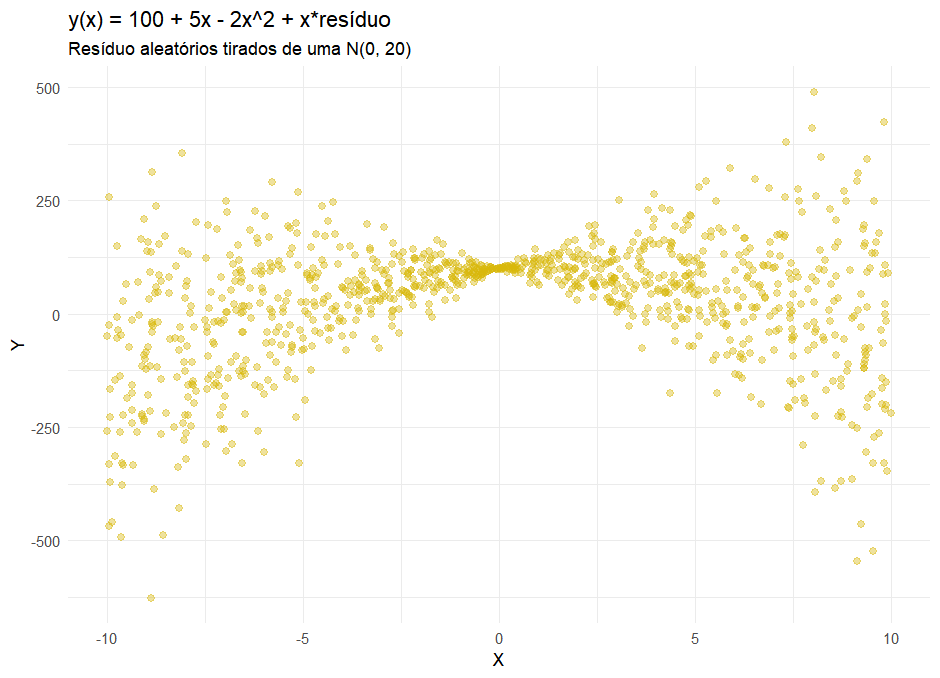
\includegraphics[scale = .75]{imagens/exemplo_heteroske.png}}
    \fonte{Elaboração própria.}
\end{figure}

\begin{table}

\caption{\label{tab:tabela_hetero}Modelo com termo quadrático. Elaboração própria.}
\centering
\begin{tabular}[t]{l|r|r|r}
\hline
termo & estimativa & erro\_padrao & estatistica\_t\\
\hline
(Intercept) & 97.64 & 6.97 & 14.01\\
\hline
x & 24.72 & 3.15 & 7.86\\
\hline
x2 & -2.37 & 0.30 & -7.95\\
\hline
\end{tabular}
\end{table}


Agora quando tentamos recuperar os parâmetros obtemos estimativas estatisticamente significantes, como informa a Tabela \ref{tab:tabela_hetero}. Os parâmetros estimados, no entanto, estão à dezenas de desvios-padrão dos verdadeiros, como mostramos na Figura 6.


\end{exemplo}



% Dadas as Condições de Gauss-Markov e uma amostra $(\mathbf{X}, \mathbf{y})$, se $(\mathbf{x}_i, \mathbf{y}_i)$ são i.i.d vale que $ \E[\epsilon_i^2\, |\, \mathbf{X} ] = \E[\epsilon_i^2\, |\, \mathbf{x}_i ]  $.


\section{Efeitos Marginais}
\subsection{Em Modelos Lineares}
A primeira hipótese, Linearidade, é a chave aqui. A resposta, supomos, varia linearmente nos regressores. Podemos introduzir algumas interações criando variáveis novas que são funções não-lineares das variáveis originais, adicionamos logaritmos, potências, indicadoras e outras tantas transformações para acomodar não-linearidades. Essa abordagem promissora, no entanto, necessariamente diminui a precisão da estimativa de todos os parâmetros e seus graus de liberdade, impondo restrições.

Mesmo que essa perda de precisão seja tolerável, esbarramos em um problema embutido na construção desses modelos. Estimamos um escalar para descrever o efeito marginal de uma variável sobre a resposta e apenas isso. Estamos supondo por definição que os efeitos marginais são iguais em todo o suporte e para qualquer nível dos outros regressores. Essa hipótese, no entanto, não está presente em florestas aleatórias.

\subsection{Em Florestas Aleatórias}

Suponha que temos uma árvore treinada $\A$ e uma observação $x$. Com alguma licença poética nos referimos à previsão dessa árvore para essa obervação como $\A(x)$. De maior incômodo para o econometrista é que não é claro o que exatamente é a derivada dessa função. Isso é um problema porque boa parte da utilidade de um modelo (linear) estimado é ter um vetor de parâmetros intuitivamente interpretáveis, pois contém as derivadas parciais do modelo. 

A derivada de $\A(\cdot)$, seja lá como for, não é tão informativa. Uma pertubação em uma observação $x$ só altera o resultado da previsão de uma árvore se for grande o suficiente para deslocar $x$ para outra regra de classificação/previsão. Teríamos uma função que é nula em boa parte de seu domínio, descontínua onde não for. 

O problema é atenuado com uma floresta aleatória. Uma pertubação pequena em $x$ pode alterar a previsão de uma fração das árvores da florestas. Com um número suficientemente grande de árvores uma variação arbitrariamente pequena em $x$ leva à uma variação arbitrariamente pequena em $\F(x)$ e vale alguma forma de continuidade. 

Esse caminho sugere uma estratégia promissora. Podemos perturbar uma observação de referência e as previsões de seus vizinhos. Isso gera uma curva relacionando valores de um regressor, dado um vetor níveis para os outros regressores, às previsões. Sua inclinação nos dá os efeitos marginais, que ao contrário do que acontece em modelos lineares, são sensíveis aos níveis dos regressores que não estamos perturbando.

\section{Um Procedimento de Computação}

Suponha um modelo $\M : \X \to \Y$. Como computamos seus efeitos marginais de maneira agnóstica? Gostaríamos de aplicar um mesmo procedimento e identificar os efeitos marginais sem depender da mecânica particular de uma classe de modelos. Por trás dos panos cada classe opera um maquinário completamente diferente: redes neurais são composições sucessivas de transformações lineares, modelos lineares são polinômios, máquinas de vetores de suporte calculam distâncias de vetores a um hiperplano estimado com base nos dados. 

Se as mecânicas internas de $\M$ variam demais para termos um procedimento uniforme, podemos olhar onde não há variação entre classes de modelos, $\X$ e $\Y$. Observando os valores que as predições do modelo dão para a resposta $Y$ em uma curva parametrizada $t \in \X$ basta computar a sua derivada para achar os efeitos marginais na curva. 

Como normalmente estamos interessados no efeito de tratamento individual de uma variável, talvez seu efeito conjunto com outra, o problema é limitado a avaliar o modelo ao longo de uma ou duas dimensões apenas. Avaliar o efeito marginal de mais variáveis implica apenas repetir o procedimento, não sofrer da maldição da dimensionalidade. Esse procedimento é computacionalmente simples, barato e agnóstico ao modelo.
